\documentclass[12pt,letterpaper,titlepage]{article}

\usepackage{fontspec}
\defaultfontfeatures{Mapping=tex-text}
\usepackage{xunicode}
\usepackage{xltxtra}
\usepackage{amsmath}
\usepackage{pdfpages}
\usepackage{amsfonts}
\usepackage{bbold}
\usepackage{amssymb}
\setcounter{secnumdepth}{0}
\usepackage{nameref}
\usepackage{enumitem}
\usepackage{environ}
\usepackage{pgfplots}

\showboxdepth=\maxdimen
\showboxbreadth=\maxdimen


\usepackage{paracol}
\usepackage{wrapfig}
\globalcounter{table}
\globalcounter{figure}
\usepackage{graphicx}
\usepackage[left=1in,right=1in,top=1in,bottom=1in]{geometry}
\graphicspath{{img/}}

\author{Jacob Abel}
\title{	Exam 2 Proposed Problems
	\\\large ECE2204 CRN:82929
}

\setlength{\parskip}{0.5em}

\begin{document}
\maketitle
\begin{raggedright}

\section{Problem 1: } 
\subsection{Design}

Design the circuit below such that the rectifier has a ripple voltage of $V_r \leq 0.05V$ and output voltage of $V_o = 12V$. Then calculate the max and min rectifier output voltages $V_o^+$ and $V_o^-$. At the max and min rectifier output voltages, determine the mode and calculate the drain voltage $V_d$, the source voltage $V_s$, and the drain current $I_d$. 

Assume 
the input voltage is $V_{in} = 120V(\text{rms}) 60Hz \text{AC}$, and 
the diode has a forward voltage $V_\gamma = 1.2V$.
Assume the eNMOS transistor has 
a threshold voltage $V_T = 0.65V$,
a Width-Length ratio of $\frac{W}{L} = 2$, and
a transistor constant $K_n^\prime = 0.25mA/V^2$.
Assume the resistor values are 
$R_1 = 7k\Omega$, 
$R_2 = 17k\Omega$, 
$R_S = 4k\Omega$, and 
$R_D = 12k\Omega$.

\begin{center}
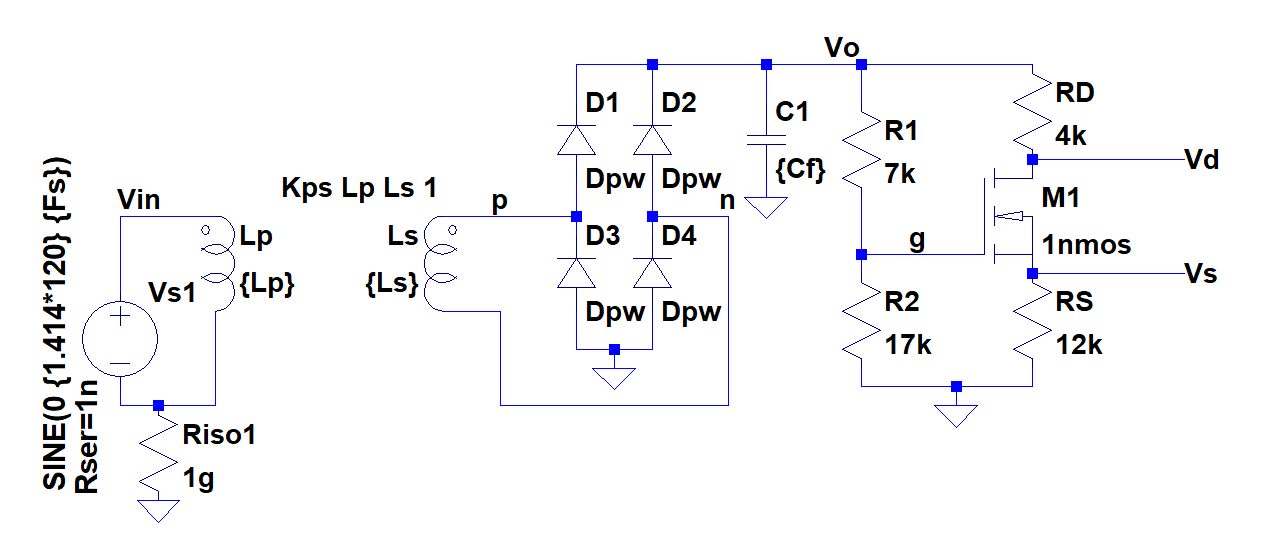
\includegraphics[width=\textwidth, height=\textheight, keepaspectratio=true]{ds1}
\end{center}


\begin{align*}
   V_{Step}
   &= \frac{V_{in}}{10}
    = 12V(\text{rms}) 60Hz \text{AC} 
\\ V_S{max} 
   &= |V_{step}(max)| + 2V_\gamma
    = |12V| + 2 \times 1.2V
    = 14.4V
\\ V_{Srms}
   &= \frac{14.4V}{2\sqrt{2}}
	= 10.18V
\\ Tr
   &= \frac{120V}{10.18V}
	= 11.79
\\ R_{Th}
   &= \frac{(R1+R2)(RS+RD)}{R1+R2+RS+RD}
	= \frac{(7k\Omega + 17k\Omega)(4k\Omega + 12k\Omega)}{7k\Omega + 17k\Omega+4k\Omega + 12k\Omega}
	= 9.6k\Omega
\\ Cf
   &= \frac{V_M}{2fRV_r}
    = \frac{12V}{2(60Hz)(9.6k\Omega)(0.05V)}
    = 0.208mF
\\ V_o^+
   &= V_M
    = 12V
\\ V_o^-
   &= V_M - V_r
    = 12V - 0.05V
    = 11.95V
\end{align*}
\begin{align*}
   V_G^+
    &= \frac{R_2}{R_1 + R_2}(V_o^+)
     = \frac{17k\Omega}{7k\Omega+17k\Omega}(12V)
     = 8.5V
\\ V_{GS}^+
    &= V_G^+ - I_D^+R_S
     = 8.5V - 12k\Omega I_D^+
\\ I_D
	&= \frac{K_n^\prime}{2}\frac{W}{L} (V_{GS}^+ - V_{T})^2
	 = 0.25 mA/V^2 (8.5V - 12k\Omega I_D - 0.65V)^2
\\	&= 532.54\mu A \text{OR} 803.57\mu A
\\ V_o^+
	&= V_D^+ + V_{DS}^+ + V_{S}^+
	 = V_{DS}^+ + I_D^+R_S + I_D^+R_D
	 = V_{DS}^+ + I_D^+(R_S + R_D)
\\ V_{DS}^+(sat)
	&= V_{GS}^+ - V_T
\\	&= 8.5V - 12k\Omega (532.54\mu A) - 0.65V
	 = 1.5V
\\	&= 8.5V - 12k\Omega (803.57\mu A) - 0.65V
	 = -1.8V
\\ V_{DS}^+
	&= V_o^+ - I_D^+(R_S + R_D)
\\  &= 12V - (532.54\mu A)(4k\Omega + 12k\Omega)
	 = 3.479V
\\  &= 12V - (803.57\mu A)(4k\Omega + 12k\Omega)
	 = -0.857V
\end{align*}
$3.479V > 1.5V$ and therefore the transistor is in saturation mode for $V_o^+$.
\begin{align*}
   I_D^+
   &= 532.54\mu A
\\ V_S^+
   &= I_D^+R_S
    = (532.54\mu A)(12k\Omega)
    = 6.39V
\\ V_D^+
   &= V_S^+ + V_{DS}^+
    = 6.39V + 3.479V
    = 9.869V
\end{align*}
\begin{align*}
   V_G^-
    &= \frac{R_2}{R_1 + R_2}(V_o^+)
     = \frac{17k\Omega}{7k\Omega+17k\Omega}(11.95V)
     = 8.46V
\\ V_{GS}^-
    &= V_G^- - I_DR_S
     = 8.46V - 12k\Omega I_D
\\ I_D
	&= \frac{K_n^\prime}{2}\frac{W}{L} (V_{GS}^- - V_{T})^2
	 = 0.25 mA/V^2 (8.46V - 12k\Omega I_D - 0.65V)^2
\\	&= 529.55\mu A \text{OR} 799.89\mu A
\\ V_{DS}^-(sat)
	&= V_{GS}^- - V_T
\\	&= 8.46V - 12k\Omega (529.55\mu A) - 0.65V
	 = 1.46V
\\ V_{DS}^-
	&= V_o^- - I_D^-(R_S + R_D)
\\  &= 12V - (529.55\mu A)(4k\Omega + 12k\Omega)
	 = 3.527V
\end{align*}
$3.527V > 1.46V$ and therefore the transistor is in saturation mode for $V_o^-$.
\begin{align*}
   I_D^-
   &= 529.55\mu A
\\ V_S^-
   &= I_D^-R_S
    = (529.55\mu A)(12k\Omega)
    = 6.355V
\\ V_D^+
   &= V_S^- + V_{DS}^-
    = 6.355V + 3.527V
    = 9.882V
\end{align*}

The final circuit has a transformer ratio of $tr = 11.79$, a capacitor with $C = 208\mu F$, $V_o^+ = 12V$, $I_D^+ = 532.54\mu A$, $V_S^+ = 6.39V$, $V_D^+ = 9.869V$, $V_o^- = 11.95V$, $I_D^- = 529.55\mu A$, $V_S^- = 6.355V$, and $V_D^+ = 9.882V$.

\subsection{Validation}

\begin{center}
LTSpice Implementation

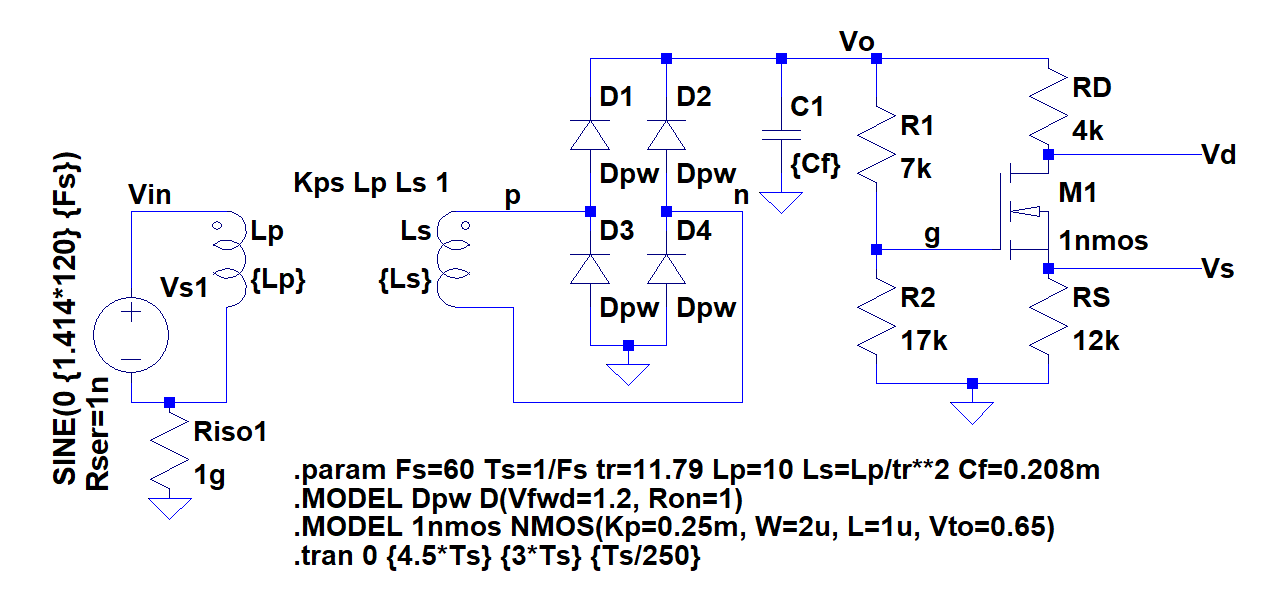
\includegraphics[width=\textwidth, height=\textheight, keepaspectratio=true]{ds1b}

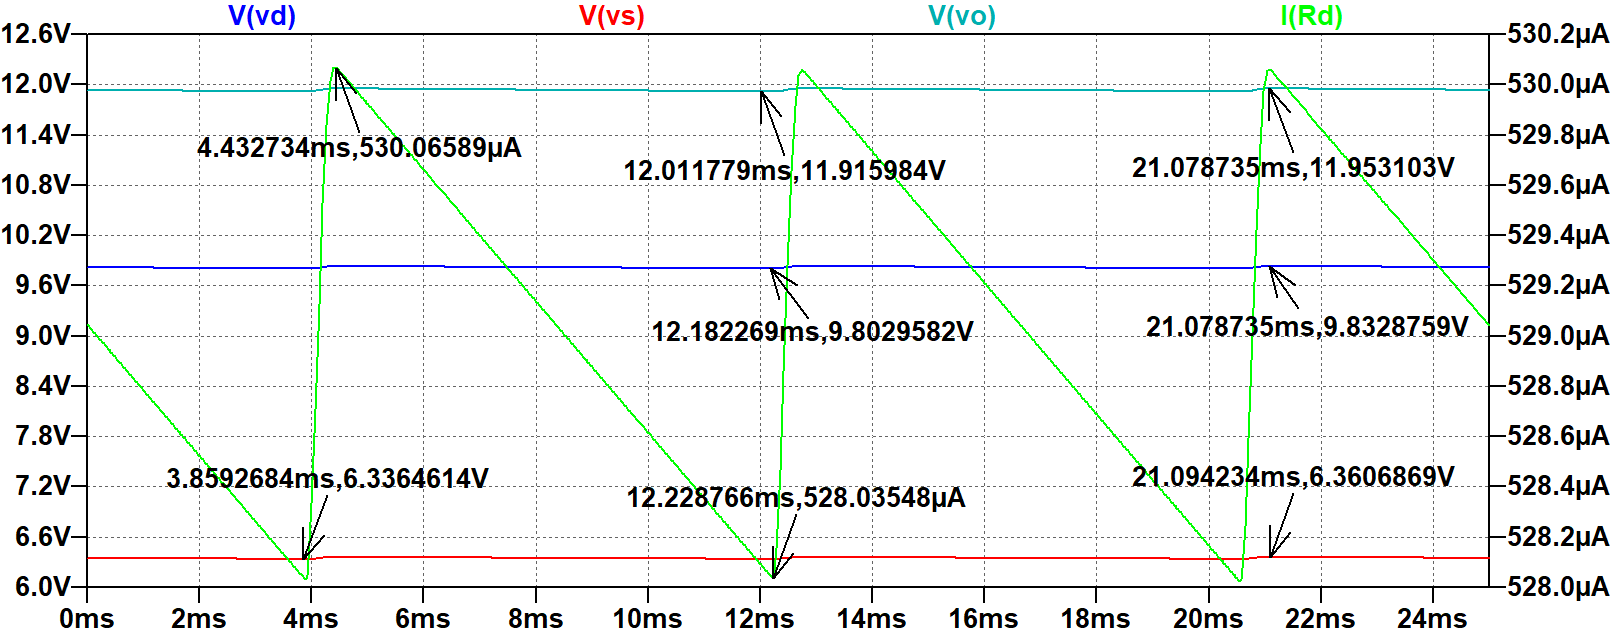
\includegraphics[width=\textwidth, height=\textheight, keepaspectratio=true]{ds1c}

\end{center}
\clearpage

\section{Problem 2: } 
Determine the mode of the eNMOS transistor from the cross section shown below with a brief justification.

\begin{center}
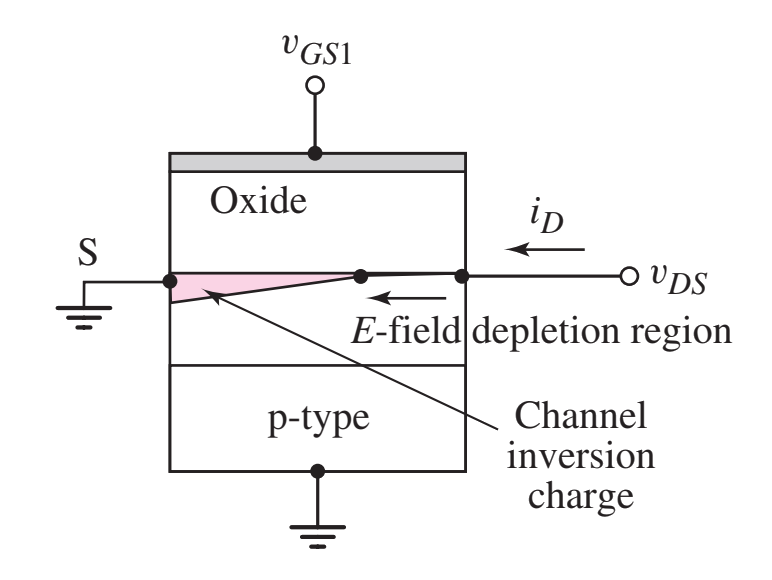
\includegraphics[width=.4\textwidth, height=\textheight, keepaspectratio=true]{ds2}
\end{center}

The transistor is in saturation mode as the channel inversion charge's path is pinched and therefore the current will be restricted and will not be able to linearly increase with the voltage. 

\end{raggedright}
\end{document}
